
%<<setup-child, include = FALSE>>=
%library(knitr)
%library(microbenchmark)
%library(reshape2)
%library(ggplot2)
%set_parent("../style/preamble.Rnw")

%set.seed(1)
%@

\input{../../2021/style/preamble4tex}
% dependencies: amsmath, amssymb, dsfont
% math spaces
\ifdefined\N
\renewcommand{\N}{\mathds{N}} % N, naturals
\else \newcommand{\N}{\mathds{N}} \fi
\newcommand{\Z}{\mathds{Z}} % Z, integers
\newcommand{\Q}{\mathds{Q}} % Q, rationals
\newcommand{\R}{\mathds{R}} % R, reals
\ifdefined\C
\renewcommand{\C}{\mathds{C}} % C, complex
\else \newcommand{\C}{\mathds{C}} \fi
\newcommand{\continuous}{\mathcal{C}} % C, space of continuous functions
\newcommand{\M}{\mathcal{M}} % machine numbers
\newcommand{\epsm}{\epsilon_m} % maximum error

% counting / finite sets
\newcommand{\setzo}{\{0, 1\}} % set 0, 1
\newcommand{\setmp}{\{-1, +1\}} % set -1, 1
\newcommand{\unitint}{[0, 1]} % unit interval

% basic math stuff
\newcommand{\xt}{\tilde x} % x tilde
\newcommand{\argmin}{\mathop{\mathrm{arg\,min}}} % argmin
\newcommand{\argmax}{\mathop{\mathrm{arg\,max}}} % argmax
\newcommand{\argminlim}{\argmin\limits} % argmin with limits
\newcommand{\argmaxlim}{\argmax\limits} % argmax with limits
\newcommand{\sign}{\operatorname{sign}} % sign, signum
\newcommand{\I}{\mathbb{I}} % I, indicator
\newcommand{\order}{\mathcal{O}} % O, order
\newcommand{\bigO}{\mathcal{O}} % Big-O Landau
\newcommand{\littleo}{{o}} % Little-o Landau
\newcommand{\pd}[2]{\frac{\partial{#1}}{\partial #2}} % partial derivative
\newcommand{\floorlr}[1]{\left\lfloor #1 \right\rfloor} % floor
\newcommand{\ceillr}[1]{\left\lceil #1 \right\rceil} % ceiling
\newcommand{\indep}{\perp \!\!\! \perp} % independence symbol

% sums and products
\newcommand{\sumin}{\sum\limits_{i=1}^n} % summation from i=1 to n
\newcommand{\sumim}{\sum\limits_{i=1}^m} % summation from i=1 to m
\newcommand{\sumjn}{\sum\limits_{j=1}^n} % summation from j=1 to p
\newcommand{\sumjp}{\sum\limits_{j=1}^p} % summation from j=1 to p
\newcommand{\sumik}{\sum\limits_{i=1}^k} % summation from i=1 to k
\newcommand{\sumkg}{\sum\limits_{k=1}^g} % summation from k=1 to g
\newcommand{\sumjg}{\sum\limits_{j=1}^g} % summation from j=1 to g
\newcommand{\summM}{\sum\limits_{m=1}^M} % summation from m=1 to M
\newcommand{\meanin}{\frac{1}{n} \sum\limits_{i=1}^n} % mean from i=1 to n
\newcommand{\meanim}{\frac{1}{m} \sum\limits_{i=1}^m} % mean from i=1 to n
\newcommand{\meankg}{\frac{1}{g} \sum\limits_{k=1}^g} % mean from k=1 to g
\newcommand{\meanmM}{\frac{1}{M} \sum\limits_{m=1}^M} % mean from m=1 to M
\newcommand{\prodin}{\prod\limits_{i=1}^n} % product from i=1 to n
\newcommand{\prodkg}{\prod\limits_{k=1}^g} % product from k=1 to g
\newcommand{\prodjp}{\prod\limits_{j=1}^p} % product from j=1 to p

% linear algebra
\newcommand{\one}{\bm{1}} % 1, unitvector
\newcommand{\zero}{\mathbf{0}} % 0-vector
\newcommand{\id}{\bm{I}} % I, identity
\newcommand{\diag}{\operatorname{diag}} % diag, diagonal
\newcommand{\trace}{\operatorname{tr}} % tr, trace
\newcommand{\spn}{\operatorname{span}} % span
\newcommand{\scp}[2]{\left\langle #1, #2 \right\rangle} % <.,.>, scalarproduct
\newcommand{\mat}[1]{\begin{pmatrix} #1 \end{pmatrix}} % short pmatrix command
\newcommand{\Amat}{\mathbf{A}} % matrix A
\newcommand{\Deltab}{\mathbf{\Delta}} % error term for vectors

% basic probability + stats
\renewcommand{\P}{\mathds{P}} % P, probability
\newcommand{\E}{\mathds{E}} % E, expectation
\newcommand{\var}{\mathsf{Var}} % Var, variance
\newcommand{\cov}{\mathsf{Cov}} % Cov, covariance
\newcommand{\corr}{\mathsf{Corr}} % Corr, correlation
\newcommand{\normal}{\mathcal{N}} % N of the normal distribution
\newcommand{\iid}{\overset{i.i.d}{\sim}} % dist with i.i.d superscript
\newcommand{\distas}[1]{\overset{#1}{\sim}} % ... is distributed as ...


\begin{document}

\lecturechapter{4}{Algorithms \& Turing Machines}
\lecture{CIM1 Statistical Computing}

\begin{vbframe}{Algorithm}

The word \emph{algorithm} is a combination of the Latin word \emph{algorismus}, named after the Persian mathematician Al-Khwarizmi, and the Greek word \emph{arithmos} (number).

\lz

\begin{minipage}{0.4\textwidth}
  \begin{center}
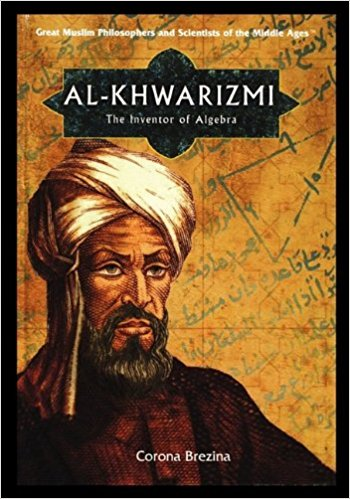
\includegraphics[width=0.7\textwidth]{figure_man/alkhwarizmi.jpg}
  \end{center}
\end{minipage}
\begin{minipage}{0.5\textwidth}
  \begin{footnotesize}
  In \emph{De numero Indorum} (about 825) Al-Khwarizmi introduced the number zero from the Indian to the Arabic number system. Furthermore, in \emph{Ludus algebrae almucgrabalaeque} (around 830) he provides a new systematic method of solving linear and quadratic systems of equations. The term algebra goes back to this work.
  \end{footnotesize}
\end{minipage}



\framebreak

What is an algorithm?

\lz

\emph{... a set of rules that precisely defines a sequence of operations such that each rule is effective and definite and such that the sequence terminates in a finite time.} \\

\lz

%What defines an algorithm?

%\begin{itemize}
%\item Uniqueness
%\item Feasibility
%\item Termination
%\item Determinacy ...
%\end{itemize}

%\framebreak

The above definition of the term algorithm is comprehensible, but mathematically inaccurate.

\lz

To receive a more precise definition, a number of approaches have been developed in the first half of the 20th century.

\lz

With the help of the \textbf{turing machine} the term can be specified much more precisely.

\end{vbframe}

\begin{vbframe}{Turing machines and algorithms}

\begin{center}
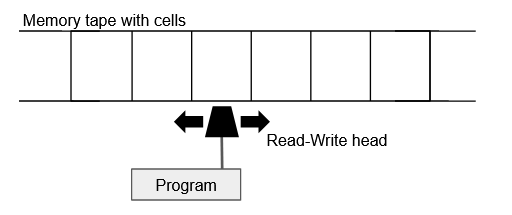
\includegraphics[width=0.5\textwidth]{figure_man/turingmachine.png}
\end{center}

A turing machine consists of

\begin{itemize}
\item a control unit that contains the program,
\item an infinitely long memory tape with discrete fields or cells,
\item a program controlled read-and-write head.
\end{itemize}


\framebreak

In each step, the turing machine changes to a new state defined in the program. The read-and-write head

\begin{itemize}
\item reads or scans the current symbol,
\item overwrites it,
\item moves a field to the left or right or stops.
\end{itemize}

The \textbf{number} of states is \textbf{finite}. The turing machine stops if no transition to a new state is defined for the current state and the symbol read from the current cell.


\framebreak

Using the concept of the turing machine we define:

\begin{center}
\begin{minipage}{0.9\textwidth}
\emph{A calculation rule for solving a problem is called an algorithm if there exists an equivalent turing machine for this calculation rule which stops for every input that has a solution.} \\
\end{minipage}
\end{center}

If a (terminating) algorithm exists, the problem is called \textbf{computable}.

\lz

\textbf{Examples: }

\begin{itemize}
\item Computable: determination of the $n$-th member of the Fibonacci sequence
\item Non-computable: The Halting problem (Problem of determining from a description of an arbitrary computer program and an input whether the program will finish running or continue to run forever)
\end{itemize}

\framebreak

The field of computability theory deals in particular with the question which problems are computable. In computer science it is usually assumed that the \textbf{Church-Turing thesis}

\begin{center}
\begin{minipage}{0.9\textwidth}
\emph{The class of turing-computable functions corresponds to the class of intuitively computable functions. } \\
\end{minipage}
\end{center}

holds. Since the term \enquote{intuitively computable function} cannot be formalized, the thesis cannot be proved.

\vfill

\begin{footnotesize}
Computability can also be defined equivalently on the basis of other equally powerful models of computation such as register machines or the lambda calculus. Due to their structural simplicity, turing machines are usually chosen in computability theory.
\end{footnotesize}

\framebreak

\textbf{Example} for a turing machine: Addition of 1

\tikzset{every loop/.style={min distance=10mm,in=-320,out=-220,looseness=10}}

% Turing machine
% Author: Sebastian Sardina
\begin{figure}[widht=0.6\textwidth]
  \begin{tikzpicture}
  \tikzstyle{every path}=[thick]

  \edef\sizetape{0.7cm}
  \tikzstyle{tmtape}=[draw,minimum size=\sizetape]
  \tikzstyle{tmhead}=[arrow box,draw,minimum size=.5cm,arrow box
  arrows={east:.25cm, west:0.25cm}]

  %% Draw TM tape
  \begin{scope}[start chain=1 going right,node distance=-0.15mm]
  \node [on chain=1,tmtape,draw=none] {$\ldots$};
  \node [on chain=1,tmtape] {};
  \node [on chain=1,tmtape] (input) {1};
  \node [on chain=1,tmtape] {0};
  \node [on chain=1,tmtape] {1};
  \node [on chain=1,tmtape] {1};
  \node [on chain=1,tmtape] {};
  \node [on chain=1,tmtape] {};
  \node [on chain=1,tmtape,draw=none] {$\ldots$};
  \node [on chain=1] {};
  \end{scope}

  %% Draw TM Program
  \begin{scope}
  [shift={(3cm,-1.5cm)},start chain=circle placed {at=(-\tikzchaincount*60:1.5)}]

  % Arrow to current state
  \node (fsbox)
  {};
  \end{scope}

  %% Draw TM head below (input) tape cell
  \node [tmhead,yshift=-.3cm] at (input.south) (head) {$s_0$};
  \end{tikzpicture}

  \begin{footnotesize}
  \begin{tabular}{|c|c|c|c|c|}
    \hline
    \textbf{State} & \textbf{Symbol read} & \textbf{Write} & \textbf{Move} & \textbf{Next state} \\
    \hline
    $s_0$ & Blank & Blank & $\leftarrow$ & $s_1$ \\
    $s_0$ & $0$ & $0$ & $\rightarrow$ & $s_0$ \\
    $s_0$ & $1$ & $1$ &  $\rightarrow$ & $s_0$ \\
    \hline
    $s_1$ & Blank & $1$ & $\leftarrow$ & $s_2$ \\
    $s_1$ & $0$ & $1$ & $\leftarrow$ & $s_2$ \\
    $s_1$ & $1$ & $0$ &  $\leftarrow$ & $s_1$ \\
    \hline
    $s_2$ & Blank & Blank & $\rightarrow$ & Stop \\
    $s_2$ & $0$ & $0$ & $\leftarrow$ & $s_2$ \\
    $s_2$ & $1$ & $1$ &  $\leftarrow$ & $s_2$ \\
    \hline
  \end{tabular}
  \end{footnotesize}
\end{figure}

\begin{footnotesize}
\href{http://turingmaschine.klickagent.ch/einband}{\color{blue}\underline{Interactive example implementation}} of different basic operations
\end{footnotesize}

\framebreak

\begin{figure}[width=0.6\textwidth]
	\begin{tikzpicture}
	\tikzstyle{every path}=[thick]
	
	\edef\sizetape{0.7cm}
	\tikzstyle{tmtape}=[draw,minimum size=\sizetape]
	\tikzstyle{tmhead}=[arrow box,draw,minimum size=.5cm,arrow box
	arrows={east:.25cm, west:0.25cm}]
	
	%% Draw TM tape
	\begin{scope}[start chain=1 going right,node distance=-0.15mm]
	\node [on chain=1,tmtape,draw=none] {$\ldots$};
	\node [on chain=1,tmtape] {};
	\node [on chain=1,tmtape] (input) {1};
	\node [on chain=1,tmtape] (second) {0};
	\node [on chain=1,tmtape] (third) {1};
	\node [on chain=1,tmtape] (fourth) {1};
	\node [on chain=1,tmtape] (blank_right) {};
	\node [on chain=1,tmtape] {};
	\node [on chain=1,tmtape,draw=none] {$\ldots$};
	\node [on chain=1] {};
	\end{scope}
	
	%% Draw TM Program
	\begin{scope}
	[shift={(3cm,-1.5cm)},start chain=circle placed {at=(-\tikzchaincount*60:1.5)}]
	
	% Arrow to current state
	\node (fsbox)
	{};
	\end{scope}
	
	%% Draw TM head below (input) tape cell
	\node [tmhead,yshift=-.3cm] at (blank_right.south) (head) {$s_0$};
	\end{tikzpicture}
	
	\begin{tikzpicture}
	\tikzstyle{every path}=[thick]
	
	\edef\sizetape{0.7cm}
	\tikzstyle{tmtape}=[draw,minimum size=\sizetape]
	\tikzstyle{tmhead}=[arrow box,draw,minimum size=.5cm,arrow box
	arrows={east:.25cm, west:0.25cm}]
	
	%% Draw TM tape
	\begin{scope}[start chain=1 going right,node distance=-0.15mm]
	\node [on chain=1,tmtape,draw=none] {$\ldots$};
	\node [on chain=1,tmtape] {};
	\node [on chain=1,tmtape] (input) {1};
	\node [on chain=1,tmtape] (second) {0};
	\node [on chain=1,tmtape] (third) {1};
	\node [on chain=1,tmtape] (fourth) {1};
	\node [on chain=1,tmtape] (blank_right) {};
	\node [on chain=1,tmtape] {};
	\node [on chain=1,tmtape,draw=none] {$\ldots$};
	\node [on chain=1] {};
	\end{scope}
	
	%% Draw TM Program
	\begin{scope}
	[shift={(3cm,-1.5cm)},start chain=circle placed {at=(-\tikzchaincount*60:1.5)}]
	
	% Arrow to current state
	\node (fsbox)
	{};
	\end{scope}
	
	%% Draw TM head below (input) tape cell
	\node [tmhead,yshift=-.3cm] at (fourth.south) (head) {$s_1$};
	\end{tikzpicture}
	
	\begin{footnotesize}
	\begin{tabular}{|c|c|c|c|c|}
		\hline 
		\textbf{State} & \textbf{Symbol read} & \textbf{Write} & \textbf{Move} & \textbf{Next state} \\ 
		\hline 
		$s_0$ & Blank & Blank & $\leftarrow$ & $s_1$ \\ 
		$s_0$ & $0$ & $0$ & $\rightarrow$ & $s_0$ \\
		$s_0$ & $1$ & $1$ &  $\rightarrow$ & $s_0$ \\
		\hline 
		$s_1$ & Blank & $1$ & $\leftarrow$ & $s_2$ \\ 
		$s_1$ & $0$ & $1$ & $\leftarrow$ & $s_2$ \\
		$s_1$ & $1$ & $0$ &  $\leftarrow$ & $s_1$ \\
		\hline 
		$s_2$ & Blank & Blank & $\rightarrow$ & Stop \\ 
		$s_2$ & $0$ & $0$ & $\leftarrow$ & $s_2$ \\
		$s_2$ & $1$ & $1$ &  $\leftarrow$ & $s_2$ \\
		\hline 
	\end{tabular} 
	\end{footnotesize}
	
\end{figure}

\framebreak

\begin{figure}
	\begin{tikzpicture}
	\tikzstyle{every path}=[thick]
	
	\edef\sizetape{0.7cm}
	\tikzstyle{tmtape}=[draw,minimum size=\sizetape]
	\tikzstyle{tmhead}=[arrow box,draw,minimum size=.5cm,arrow box
	arrows={east:.25cm, west:0.25cm}]
	
	%% Draw TM tape
	\begin{scope}[start chain=1 going right,node distance=-0.15mm]
	\node [on chain=1,tmtape,draw=none] {$\ldots$};
	\node [on chain=1,tmtape] {};
	\node [on chain=1,tmtape] (input) {1};
	\node [on chain=1,tmtape] (second) {0};
	\node [on chain=1,tmtape] (third) {0};
	\node [on chain=1,tmtape] (fourth) {0};
	\node [on chain=1,tmtape] (blank_right) {};
	\node [on chain=1,tmtape] {};
	\node [on chain=1,tmtape,draw=none] {$\ldots$};
	\node [on chain=1] {};
	\end{scope}
	
	%% Draw TM Program
	\begin{scope}
	[shift={(3cm,-1.5cm)},start chain=circle placed {at=(-\tikzchaincount*60:1.5)}]
	
	% Arrow to current state
	\node (fsbox)
	{};
	\end{scope}
	
	%% Draw TM head below (input) tape cell
	\node [tmhead,yshift=-.3cm] at (second.south) (head) {$s_1$};
	\end{tikzpicture}
	
	\begin{tikzpicture}
	\tikzstyle{every path}=[thick]
	
	\edef\sizetape{0.7cm}
	\tikzstyle{tmtape}=[draw,minimum size=\sizetape]
	\tikzstyle{tmhead}=[arrow box,draw,minimum size=.5cm,arrow box
	arrows={east:.25cm, west:0.25cm}]
	
	%% Draw TM tape
	\begin{scope}[start chain=1 going right,node distance=-0.15mm]
	\node [on chain=1,tmtape,draw=none] {$\ldots$};
	\node [on chain=1,tmtape] {};
	\node [on chain=1,tmtape] (input) {1};
	\node [on chain=1,tmtape] (second) {1};
	\node [on chain=1,tmtape] (third) {0};
	\node [on chain=1,tmtape] (fourth) {0};
	\node [on chain=1,tmtape] (blank_right) {};
	\node [on chain=1,tmtape] {};
	\node [on chain=1,tmtape,draw=none] {$\ldots$};
	\node [on chain=1] {};
	\end{scope}
	
	%% Draw TM Program
	\begin{scope}
	[shift={(3cm,-1.5cm)},start chain=circle placed {at=(-\tikzchaincount*60:1.5)}]
	
	% Arrow to current state
	\node (fsbox)
	{};
	\end{scope}
	
	%% Draw TM head below (input) tape cell
	\node [tmhead,yshift=-.3cm] at (input.south) (head) {$s_2$};
	\end{tikzpicture}
	
	\begin{footnotesize}
	\begin{tabular}{|c|c|c|c|c|}
		\hline 
		\textbf{State} & \textbf{Symbol read} & \textbf{Write} & \textbf{Move} & \textbf{Next state} \\ 
		\hline 
		$s_0$ & Blank & Blank & $\leftarrow$ & $s_1$ \\ 
		$s_0$ & $0$ & $0$ & $\rightarrow$ & $s_0$ \\
		$s_0$ & $1$ & $1$ &  $\rightarrow$ & $s_0$ \\
		\hline 
		$s_1$ & Blank & $1$ & $\leftarrow$ & $s_2$ \\ 
		$s_1$ & $0$ & $1$ & $\leftarrow$ & $s_2$ \\
		$s_1$ & $1$ & $0$ &  $\leftarrow$ & $s_1$ \\
		\hline 
		$s_2$ & Blank & Blank & $\rightarrow$ & Stop \\ 
		$s_2$ & $0$ & $0$ & $\leftarrow$ & $s_2$ \\
		$s_2$ & $1$ & $1$ &  $\leftarrow$ & $s_2$ \\
		\hline 
	\end{tabular} 
	\end{footnotesize}
	
\end{figure}

\end{vbframe}

%\begin{vbframe}{Efficiency of algorithms}

%We are interested in the \textbf{efficiency} of algorithms. Efficiency can be associated with different attributes such as
%  \begin{itemize}
%    \item CPU runtime
%    \item Memory usage
%    \item Memory usage on the hard drive
%  \end{itemize}

%\lz

%We will mainly focus on the \textbf{runtime behavior} of algorithms.

%\end{vbframe}

\begin{vbframe}{Algorithms and elementary operations}

\begin{itemize}
\item We can theoretically describe the runtime of an algorithm by using turing machines and counting the number of steps a turing machine needs to solve the problem.
\item However, it is usually sufficient to consider an algorithm - less precise but more intuitive - as a \textbf{list of instructions}.
\item Using this definition, we can \enquote{measure} the runtime by counting the number of \enquote{elementary operations} performed.
\item An elementary operation is a step that does \textbf{not} depend on the size of the problem.
\item This distinction makes it easier for us to measure the runtime of an algorithm.
\end{itemize}

\framebreak

For simplicity, we assume that the time needed to evaluate a function is \textbf{proportional} to the number of \enquote{elementary operations} performed.

\lz

Examples of elementary operations:

\begin{itemize}
  \item An arithmetic operation, e.g. \code{x + y}
  \item An assignment, e.g. \code{x = 1}
  \item A test, e.g. \code{x == 3}
\end{itemize}

\framebreak

\textbf{Caution:}
\begin{itemize}
\item Strictly speaking, the runtime of arithmetic operations depends on the problem, e.g. when adding $x + y$, it depends on the size of the numbers $x, y$.
\item Nevertheless, we count each arithmetic operation as one step and assume that the runtime of the operation is not influenced by the number itself.
\item In most cases this is not a problem, since the size of the numbers does not grow systematically as the algorithm progresses.
\item However, there are exceptions where the complexity depends significantly on the size of the number (e.g., testing whether a number is a prime). Here one would use a different calculation model such as the number of bit operations.
\end{itemize}

\end{vbframe}

\begin{vbframe}{Runtime Growth (Example)}
Let's say you want to check if integer \code{x} is a \textbf{prime number}!

\lz

For solving the problem you use two different algorithms:
\begin{enumerate}
  \item The first algorithm divides \code{x} by every integer from 2 to \code{x-1} to determine its divisibility.
  \item The second algorithm divides \code{x} by every integer from 2 to \code{sqrt(x)} to determine its divisibility.
\end{enumerate}

\lz

Both algorithms will provide the correct result*, but while the number of basic operations in algorithm~1 is \code{x-2}, the number of basic operations in algorithm~2 is \code{< sqrt(x)} and hence for \code{x > 4} algorithm~2 is much faster and its runtime grows much slower!

\lz

\begin{footnotesize}
*Obviously, if $x_1 > sqrt(x)$, then $x_2 = x / x_1$ results in $x_2 < sqrt(x)$ so you just have to check the integers $\le sqrt(x)$!
\end{footnotesize}

\end{vbframe}



\endlecture
\end{document}
